\documentclass[tikz,border=12pt]{standalone}
\usepackage[T1]{fontenc}
\usepackage{mathpazo}
\usepackage{pgfplots}
\usepgfplotslibrary{groupplots}
\pgfplotsset{compat=1.18}

\definecolor{morblue}{HTML}{7b97ad}
\definecolor{morlavender}{HTML}{907ea0}
\definecolor{morgold}{HTML}{b8995e}
\definecolor{mortext}{HTML}{3d352f}
\definecolor{morgrid}{HTML}{e0d9d1}
\definecolor{morbg}{HTML}{faf7f3}

\begin{document}
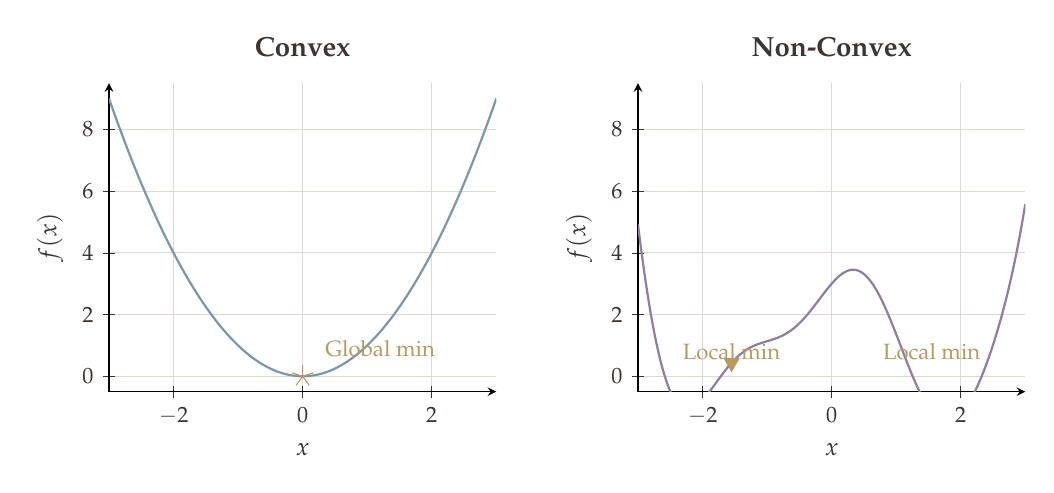
\begin{tikzpicture}
\begin{groupplot}[
  group style={
    group size=2 by 1,
    horizontal sep=1.8cm,
  },
  width=6.5cm, height=5.5cm,
  xlabel={$x$},
  ylabel={$f(x)$},
  xmin=-3, xmax=3,
  ymin=-0.5, ymax=9.5,
  axis lines=left,
  every axis label/.style={font=\small, color=mortext},
  every tick label/.style={font=\footnotesize, color=mortext},
  grid=major,
  grid style={morgrid, thin},
  tick style={mortext},
]

% Left panel: Convex
\nextgroupplot[title={\textbf{Convex}}, title style={font=\normalsize, color=mortext}]
\addplot[morblue, thick, smooth, domain=-3:3, samples=100] {x^2};
\addplot[only marks, mark=star, mark size=4pt, morgold, mark options={fill=morgold}]
  coordinates {(0,0)};
\node[morgold, font=\footnotesize, anchor=south west] at (axis cs:0.2,0.3) {Global min};

% Right panel: Non-convex
\nextgroupplot[title={\textbf{Non-Convex}}, title style={font=\normalsize, color=mortext}]
\addplot[morlavender, thick, smooth, domain=-3:3, samples=200]
  {x^4/4 - 2*x^2 + 0.8*sin(deg(3*x)) + 3};
\addplot[only marks, mark=triangle*, mark size=3pt, morgold, mark options={fill=morgold, rotate=180}]
  coordinates {(-1.55, {(-1.55)^4/4 - 2*(-1.55)^2 + 0.8*sin(deg(3*(-1.55))) + 3})
               ( 1.55, {( 1.55)^4/4 - 2*( 1.55)^2 + 0.8*sin(deg(3*( 1.55))) + 3})};
\node[morgold, font=\footnotesize, anchor=south] at (axis cs:-1.55,0.2) {Local min};
\node[morgold, font=\footnotesize, anchor=south] at (axis cs:1.55,0.2) {Local min};

\end{groupplot}
\end{tikzpicture}
\end{document}
